\chapter{Jester API Design}\label{chap:api_des}

The overarching goal of Jester is to provide an API that simplifies the process of creating applications that utilize the human skeleton for input. It needs to be easy to map data from any skeletal position API, retrieve skeleton data in a usable format, setup sensor environments, and fuse and filter sensor data. The Jester API is designed to make these processes as straight forward as possible while allowing developers to create sensor wrappers and modify the fusion and filtering processes easily. All of this functionality must be provided in an manner that minimizes the coding overhead for initializing the Jester system and does not impair the performance of the application.

\begin{figure}[]
\centering
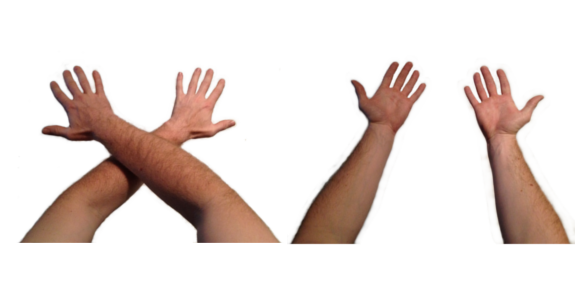
\includegraphics[width=0.5\textwidth]{figures/handAmbig}
\caption{Thumb position alone is not sufficient to disambiguate hands. Other data is required in the case of cross body reach.}
\label{fig:hand_cross}
\end{figure}

While it is possible to create a generic data fuser that merges incoming data from different sources into the same skeleton for most situations, it is not possible to create a fuser that will work for every possible system setup. For instance, the Leap Motion Controller cannot tell if the hand it is tracking is oriented palm up or palm down. This limitation means that its hand position will always be ambiguous since it cannot be sure which hand is being tracked when the user moves his hands into the the Leap’s tracking box while reaching across his body like in pose A in figure \ref{fig:hand_cross}. A second sensor is necessary if the application developer wishes to eliminate the ambiguity. In the case of the Jester sample application discussed in chapter \ref{chap:sample_app}, the PrimeSense Carmine is used to disambiguate hand position. The Carmine has long enough sensing range and a wide enough field of view to capture and track the user’s entire skeleton but does not sense wrist position as accurately as the LeapMotion Controller. A default data fusion class could easily assign a higher weight to the Leap’s wrist position and integrate the non-overlapping bones into the same skeleton. However, a true disambiguation requires the ability for the fuser to realize that the user is doing cross body reach pose A and reassign the false finger data that results from assuming the more natural pose B in figure \ref{fig:hand_cross}. Situations like this illustrate the necessity of modular and developer programmable data fusion units as well as the unfortunate reality that there cannot be a universal data fusion solution.

There are many different kinds of sensors that can be used to track different parts of the human body that all have different strengths and limitations. Most sensors have different APIs for retrieving skeletal tracking. In order for a sensor abstraction system like Jester to see wide adoption, input support for a large number of sensors and APIs is required. Since Jester is not backed by a large company and will not have full time developer support it is critical that third party developers can create and share sensor wrappers without requiring changes to the core of Jester. Unfortunately, abstraction alone is not sufficient to create a truly sensor agnostic system because an application may require data that the sensors present are not capable of providing; for example a system with only a Leap present cannot resolve the user’s head position. 

Jester’s flexibility requirements necessitate that Jester provides a sensor abstraction that allows developers to create thin wrappers for any skeletal tracking API that are distributable separately from the Jester core API as well as easily adaptable data fusion classes. This chapter will cover the core Jester functionality: the datapath, internal skeletal representation, and spatial transformation systems. It will also explain the sensor abstraction, data fusion, and data filtering architecture.

\section{Jester Core}\label{sec:jester_core}

Jester’s sensor wrappers and data fusion units need to be flexible in order to be useful. However, Jester’s core functionality and abstraction base classes should remain relatively constant in order to ensure backwards compatibility with older sensor wrapper and fusion implementations. If the abstraction interfaces are  designed correctly, the core should not need to be modified by developers. Therefore the Jester datapath, internal skeletal model, spatial transforms, and abstraction interfaces are kept separate from their implementations and are known as the Jester core. The Jester core is designed to be compiled into a library and does not need to be recompiled when new sensor wrappers or data fusion or filtering modules are created.

\subsection{Data Path}

Jester requires a data path that does not rely on sensors having any knowledge of the internal skeletal model or any other sensors that may present in order to allow sensor modules to be truly modular. So, there must be a black box style system for passing data from the sensor wrappers to the data fuser and then into the internal skeletal model. 

The data path, illustrated in figure \ref{fig:broad_datapath}, centers around a controller class. The controller is constructed with a pointer to a data fusion class factory that is chosen or implemented by the application developer and is the center of a multi-step setup process depicted in figure \ref{fig:const_order} and described here. The Jester core comes with a data fusion implementation and factory that is adequate for straightforward fusion requirements; its design and implementation are discussed in section \ref{sec:fuser_des_impl}. When the controller is constructed using the constructor depicted in figure \ref{fig:broad_datapath}, it invokes the data fusion factory and then constructs an instance of the scene class with a pointer to the factory. The scene class is the root of the hierarchical skeletal model and is responsible for constructing and providing access to the bones that make up the skeleton. The scene class functionality is explained in section \ref{sec:scene_impl}. The controller then sets the newly created scene class to be the root space of the data fusion module in order to provide a common space in which to unite measurements and allow the fuser to cooperate with the scene to resolve race conditions discussed later. The controller, and therefore the scene and skeleton, must be constructed before individual sensors because sensors are a part of the scene graph along with the skeleton. The scene graph will be thoroughly explained in section \ref{sec:bone_hierarchy}, but, briefly, placing sensors in the scene graph allows sensors to be mounted to body parts and automatically handled by the space unification system discussed in section \label{sec:bone_hierarchy}. 

Once the controller and scene are initialized, the application constructs the sensor classes for the sensors that are present in the system. Jester does not detect available sensors because there are simply too many different kinds and some setup specific manual configuration, discussed in section \ref{sec:sensor_wrappers}, is necessary. The sensor base class constructor requires pointers to the sensor’s scene graph parent and the controller. The scene graph parent pointer is necessary to provide a spatial context for the sensor measurements and will be discussed in sections \ref{sec:scene_impl}. The Jester controller provides a pair of functions called Controller::suggestBoneInfo(...) and Controller::suggestJointInfo(...) that allow the sensor class to asynchronously feed data into Jester when it arrives from the sensor API and without any knowledge of the timing issues, discussed in section \ref{sec:fuser_des_impl} that arise from having multiple sensors present in the same system.

When the Controller::suggestBoneInfo(...) or Controller::suggestJointInfo(...) are called the controller invokes the DataFusionModule::newData(...) function using the pointer to the data fusion module that was provided at the time of its construction with the same arguments that were received by the controller. The  data fusion module is responsible for storing the new skeletal data internally and fusing it asynchronously with data from other sensors in the system to form a complete skeletal model. The data storage and fusion process will be explained in section \ref{sec:fuser_des_impl}.

Once the sensor data has been fused into a cohesive skeletal model, the only remaining step is to provide access for applications. The controller provides a getter function to retrieve a pointer to the scene root class. The scene root is the parent of the skeleton and contains accessor methods to retrieve the individual bone positions. The process of initializing the Jester core and retrieving the skeleton for the first time requires less than 10 lines of code.

\subsection{Core Data Representation}

In computer graphics and animation the human skeleton is generally represented as a hierarchical model where each bone position depends on the position of the previous bone. Hierarchical modeling is a good analog to how the human skeleton actually behaves \cite{parent2012computer}. For example if a person swivels her upper arm, or humerus, at her shoulder but does not change her elbow or wrist angle the position of her hand still changes as illustrated in figure \ref{fig:arm_swivel}. Rather than marching down the chain of bones affected by the humerus and updating their 3D position every time there is a small change in parent position it is much more efficient to store each bones position relative to its parent. With relative positioning, parent position changes are automatically reflected when the child position is resolved.

Jester uses a spatial mathematics library called OpenGL Mathematics (GLM). GLM is a header only C++ library and so can be used on any system with a C++ compiler. It is designed to provide all of the functionality that a graphics application would need, and provides all of the quaternion, vector, and matrix operations needed for Jester. There are many solid math libraries, but GLM is commonly used in the graphics community because it is designed to mirror the GLSL API used in OpenGL programming \cite{glm}.

\subsubsection{Hierarchical Skeleton}\label{sec:bone_hierarchy}

In Jester, each bone stores a length, 3D start position in reference to the end of the parent, and an orientation as a quaternion with respect to the parent orientation. Each bone creates its own space where the bone runs down the positive Z axis. In order to take a point in one bone’s space and transform it to its parent’s space Jester creates a 4x4 matrix by translating an identity matrix by the bone’s starting position and then multiplying the new matrix by a rotation matrix derived from the bone orientation quaternion. The resulting matrix is known as the transform for the bone’s space and can translate any point from the bone’s space to its parent’s space. To transform a point from bone space all the way to world space, or the root space for the application, the 4x4 transforms for each bone in the hierarchy are multiplied to form one world transform. Similarly, the rotation of a bone in its parent’s space, and, by extension, world space, can be determined by multiplying the orientation quaternions together until the desired space is reached. The chaining of bone spaces can be visualized as seen in figure \ref{fig:joint_spaces}. Rendering a bone in OpenGL is as simple as rendering a cylindrical triangle mesh with a model matrix that is defined by scaling the bones world space transform by the whatever width the developer desires and the bones internally stored length.

Jester's reduced bone set maps well to the bones that can be tracked by current skeletal sensors. Figure \ref{fig:skeleton} shows the bones that have been selected. The Jester skeleton is hierarchically based on a fictional "root bone" that is is placed at the midpoint of the pelvis. A fictional bone is used because there is no centrally placed bone in the human torso that does not have other bones attached at both ends. Having children bones only placed at one end of the root allows the system to have one consistent pivot point and simplify the conceptual complexity. The head was not selected for the root because placing the head at the root would essentially rotate the entire body as the head is turned, which is not consistent with what happens in reality.

The skeletal bones themselves compose just one part of the scene graph provided by Jester. All components of the scene graph are children of the parent class Jester::SceneGraphNode. Jester::SceneGraphNode provides the base functionality for calculating the local and world position, orientation, and transform. It also tracks the node’s children and parent. Providing a generic base class for the Jester scene graph allows developers to easily incorporate the Jester scene graph into their application rather than building a custom one. If developers want to add things besides sensors to the scene graph they just have to extend the Jester::SceneGraphNode superclass. The built in scene graph inheritance is depicted in figure \ref{fig:scene_graph_inh}.

Jester’s abstract Sensor class is a subclass of Jester::SceneGraphNode. Placing Sensors in the scene graph greatly simplifies the process of merging the data from different sensors. Most sensors provide bone data with respect to their space; meaning that if the sensor is moved but the sensed bone is not the sensor will think that the bone is what moved. Similarly, two identical sensors placed side by side will track the same bones but report slightly different positions as shown in figure \ref{fig:sensor_perspective}. Most sensors are statically mounted on tabletops or walls, but it makes sense to mount some sensors on the human skeleton itself. For instance, a user could mount a hand tracking sensor on her head mounted display, like in figure \ref{fig:sensor_perspective},  so that she could turn to look at virtual objects and then interact with them naturally without worrying about the sensor field of view like she would if it was placed on a desk. Including sensors in the scene graph makes it possible to simply use the world space transform provided by Jester::SceneGraphNode to move sensed bone positions into Jester’s world space. 

\subsubsection{Scene Root}\label{sec:scene_impl}

The root of the Jester scene graph is the Jester::Scene class. It provides the base space for all scene graph nodes as well as accessor functionality for the bones that make up the skeleton. While the Jester::SceneGraphNode class provides access to an std::iterator that makes it possible to traverse the skeleton by starting at the scene root and recursively iterating over all of the children of each node, that process would be unnecessarily cumbersome if the user just wants to access a specific bone. So, the scene class provides a function called Scene::getBone(...) that takes the ID of the desired bone and returns a pointer to the correct bone object.

The scene class also cooperates with the data fuser to provide a consistent and up to date skeleton. If the data fuser actively modified the same bone objects that are in the scene, there is a possibility that applications could render an inconsistent skeleton. Since both the data fuser and applications access the skeleton in pieces and are operating concurrently in separate threads, there is an inherent race condition illustrated in figure \ref{fig:data_race}. If a single threaded client application is attempting to render the current position of the user’s right arm, it will access the position of the humerus, then the position of the radius, and then the fingers. If the data fuser updates the position of the arm before the client accesses the radius but after the position of the humerus, the bones could be rendered disconnected from each other.

Jester solves the inconsistency problem by using a double buffering approach shown in figure \ref{fig:double_buffer}. The scene holds two sets of skeletons; one for the data fuser to update and one for the client application to read. Both skeletons are updated whenever the SceneGraphNode::addChild(...) or SceneGraphNode::removeChild(...) functions are called. The data fuser notifies the scene when it is about to modify the skeleton by calling Scene::beginSkeletonUpdate() and when it is done by calling Scene::finishSkeletonUpdate(). Locking the fusion skeleton tells the scene that it should not swap the skeletons while the data fuser is in the process of changing data. Client applications call Scene::refreshSkeleton() when they want the most up to date complete skeleton. Scene::refreshSkeleton() checks if the skeleton is currently being updated. If it is, then the client thread is blocked until the data fuser is done updating or a short timeout expires. The timeout allows the client application to not stall for long if the data fuser is hanging in order to help ensure that the client UI does not lock. Once the block is released without timeout or if the skeleton was not currently being updated, the scene enables a lock in Scene::beginSkeletonUpdate() to make the fuser wait, swaps the two skeletons so that the client application gets the most up to date data and the data fuser gets a new skeleton to modify, and disables the lock in Scene::beginSkeltonUpdate() to allow the fuser to continue. Double buffering in this manner allows Jester to support multithreaded data fusion while preventing the possibility of providing an inconsistent skeleton.

\subsection{Joints}

The position of many bones in the human body can be determined using the joints that they connect. For example, the position of the radius can be completely determined using the position of the wrist and elbow joints. Many sensors, like the PrimeSense Carmine, report skeletal position using joints instead of bones. So, the Jester framework accepts skeletal data as bone position or joint position. Bone position maps directly into the Jester skeleton, but joint data requires some special handling.

Jester has convenience functions to handle the resolution of bone position from the position of two joints. The Jester::Bone class provides enumerations for all of the bones that are supported by Jester and all of the joints that can be used to define those bones as well as a map that takes a bone ID and returns the pair of joint IDs that defines it. The Jester fusion module superclass, Jester::DataFusionModule, provides a function called getBonesFromJoints(...) that resolves bone positions by looping through the bones that are supported by Jester and checking to see if the joints mapped to each bone were provided. If both Joints were provided, the function simply sets the bone to start at the start joint and terminate at the end joint. Since not all sensors provide information about all of the joints supported by Jester, it is possible that a bone could be missing one or both joints. It is useful to provide default joint positions that can be used if joints are missing. For example, if a system only uses a LeapMotion Controller, it will be able to track the user’s wrist position but not his elbow. Jester can still create a skeleton with just the wrist positions by using the default joint positions for the unmapped joints. Assuming default joint position frequently results in distorted bone lengths as shown in figure \ref{fig:distorted_bones}, but it is not possible to infer joint position without a true inverse kinematics engine. We have decided that, for Jester, it is better to provide a possibly inaccurate skeleton than to force users to have sensors tracking every joint in order to get any data.

\section{Plugin Architecture}

The Jester core provides the functionality that is not sensor or system setup dependent. The previous section touched on the design of the sensor wrapper and data fusion classes in order to explain the Jester data flow. This section will detail the design of the modular components of Jester. Sensor API interaction, sensor fusion, and data filtering are all parts of the skeletal data input process that may need to change widely for different system implementations. So, the supporting base classes are designed to provide the basics while allowing developers to easily create custom modules.

\subsection{Sensor Wrappers}\label{sec:sensor_wrappers}

The design of the Jester sensor wrappers is probably the simplest of any class in the entire system. Developers will frequently have to be able to create their own custom wrappers for different sensor APIs because there are so many, and the core concept of Jester is to be able to support as many different sensors as possible. Due to the flexibility requirements, the specific implementation of each sensor wrapper internals is completely left to the developer. The only requirements are that the developer's sensor class be a subclass of Jester::Sensor and that it delivers data to the Jester skeleton by calling Controller::suggestJointInfo(...). 

Jester::Sensor takes Jester::SceneGraphNode and Jester::Controller pointers. The Jester::SceneGraphNode is necessary because Jester::Sensor is a subclass of Jester::SceneGraphNode and designed to be placed into the scene graph. Providing a pointer to the graph node's parent at the time of construction allows the Jester core to automatically add the new sensor to its scene graph parent's list of children. The controller pointer is not used by the Sensor superclass, but the sensor wrapper implementation will need it to pass skeletal data to the Jester core. Requiring the Jester::Controller pointer as a part of the superclass implementation makes the controller requirement apparent and attempts to simplify the process of creating sensor implementations. 

Unsurprisingly, different skeletal tracking APIs require different query methods. Some allow developers to register a callback function to handle new data. Others need to be queried continuously. Whatever the data fetching method is used will be responsible for pulling skeletal bone or joint data from the device API and mapping it to the joints or bones that are supplied by the Jester API. If there is not a one to one mapping, the sensor wrapper implementation is responsible for either disregarding the data if the bone or joint has no close analogue or translating the data if it is similar. For example, the LeapMotion API senses palm position, and the closest thing in Jester is the wrist joint. Since the LeapMotion API provides a vector for the direction the hand is pointing, a developer can simply translate the palm position a small distance in the opposite direction of the hand vector to estimate wrist position. The specific implementation details of two example sensor wrappers will be discussed in the next chapter.

The client program is responsible for either detecting the sensors present in the system or providing the user with a way of selecting their system setup. Once the client has constructed the Jester controller and the correct sensor wrappers for their system they must specify the position and orientation of the sensors with respect to its parent object in the scene graph. If the sensor is placed on an immovable surface then its parent should be the scene root, and if it is mounted to a body part, like the head, then its parent should be the bone that approximates that part. The Jester::Sensor superclass exposes functions for setting the orientation and position of the sensor. The position of the scene root center is arbitrary, so it is entirely up to the application developer. As long as the sensor positions are set relative to the same 3D point and orientation, they will form a coherent skeleton. The initialization code for a specific demo application will be discussed in section \ref{sec:app_impl}, and the implementation of two sensor wrappers in sections \ref{sec:leap_impl} and \ref{sec:carmine_impl}.
	
\subsection{Sensor Fusion}\label{sec:fuser_des_impl}

Sensor fusion requirements can vary widely depending on the type of sensors present in the system. So, the Jester sensor fusion module superclass is designed to provide a base level fusion implementation that can used as is, modified slightly to fit small differences in system needs, or even completely replaced. This section will explain the design of the base implementation and the methods for making small modifications; large modifications are too diverse to enumerate and anything can be replaced since all of the Jester::SensorFusionModule methods are abstract.

The default sensor fusion module requires application developers to tell it which sensors to expect data from by calling the SensorFusionModule::registerSensor(...) function. registerSensor(...) takes the Jester::Sensor pointer to one of the sensors that is present in the system and a map that maps either a bone ID or a joint ID to a weighting scaling value. The weighting scaling value is used to decide how much to trust measurements from that sensor about that bone or joint and will be explained in more detail shortly. The data fuser is ready to handle new bone or joint position data once all of the sensors have been registered.

Jester sensor wrappers operate in separate threads, so the sensor fusion module will be responsible for handling the inherent synchronization problems that occur when different parts of the skeleton arrive at different times shown earlier in figure \ref{fig:data_race}. This becomes especially important when multiple sensors are sending data about the same bone. The SensorFusionModule::newData(...) function is called asynchronously, so it requests a lock on a skeleton modification mutex before attempting to merge the new data with the internal skeletal model. It also keeps a history of the sensor readings as a series of independent skeletons, or "skeleton frames", to help match the data between sensors temporally. Skeleton frames are their operation are illustrated in figure \ref{fig:skeleton_frames}. The fuser runs a thread that is responsible for updating the scene's skeleton. At a set interval it examines the skeleton frame history to get the best current skeleton. If the current frame does not have data about a specific bone, it looks backwards in time a user-configurable number of frames to find the most recent known position. If it finds position data, it uses it to build the skeleton, but if there is no data within the set number of frames it uses the default bone position. After setting the skeleton, it advances the history to the next frame. 

SendorFusionModule::newData(...) accepts skeletal information as either bones or joints and Jester operates internally using bones; both data input processes are illustrated in figure \ref{fig:new_data_flow}. So, joints are transformed into bone data using the bone to joint lookup map discussed in the datapath section. If there is a filtering module present the fuser sends the new bone to the filter and then replaces the sensed position with the one given by the filter. The fuser then checks if there is any information about the new bones already in the current skeletal frame. If the data has not been set yet or is from the same sensor, the new bone position is inserted. If there is data from a different sensor, then the new position is fused by interpolating between the competing bone start positions and quaternions using a weighting equating that is a combination of the confidence supplied by the sensor reading and the scaling value for that bone [math and explain]. The frame is advanced if all of the sensors have contributed to the current frame once the data is inserted and fused. 

The length of the skeleton frame history, the number of frames to go back in time when setting the scene skeleton, and the amount of time before the frame is auto-advanced are all easily configurable to match the real time needs of the system. Frequent updates are more demanding, but provide a more current system if the sensors can keep up. The new data handling process is all handled with virtual methods, so data fusion implementations can easily change the data handling for some bones while invoking the default fusion functions with others. An example of small modifications to the fusion system is given in section \ref{sec:fuser_impl}.
	
\subsection{Data Filtering}

Different data filtering methods require very different implementation details so the Jester data filtering module provides little functionality other than a public interface for invoking the filter so that filters are somewhat easily swappable. The human skeleton has more many degrees of freedom than the filtering methods investigated for this thesis can reasonably handle so we assume that there will be a filter for each bone in the body. The Jester::DataFilter base class has an abstract virtual functions for initializing the filter, DataFilter::init(), and updating the filter with the current sensed position of the bone, DataFilter::update(...). The init function is responsible for doing any setup that the filter requires and the update function passes in the best known position of the bone. The filter is responsible for updating its internal algorithm with the new data and returning the filtered bone position. A sample particle filter is implemented in section \ref{sec:filer_impl}.
